\documentclass[twocolumn,superscriptaddress,aps, floatfix]{revtex4-1}


%%%%%%%%%%%%
% Packages %
%%%%%%%%%%%%

\usepackage[utf8]{inputenc}

\usepackage{amsfonts}
\usepackage{amssymb}
\usepackage{amsmath}
\usepackage{amsthm}

\usepackage{bbold}
\usepackage{bm}
\usepackage{graphicx}
\usepackage{color}
\usepackage{hyperref}

\usepackage{caption}
\usepackage{subcaption}


%%%%%%%%%%%%
% Document %
%%%%%%%%%%%%

\begin{document}
    % ----- Title ----- %
    
    \title{\Large{INFO8010 : Neural style transfer}}
    \vspace{1cm}
    
    \author{\small{\bf Maxime Meurisse}}
    \affiliation{\texttt{m.meurisse@student.uliege.be} (\texttt{s161278})}
    
    \author{\small{\bf Adrien Schoffeniels}}
    \affiliation{\texttt{adrien.schoffeniels@student.uliege.be} (\texttt{s162843})}
    
    \author{\small{\bf Valentin Vermeylen}}
    \affiliation{\texttt{valentin.vermeylen@student.uliege.be} (\texttt{s162864})}
    
    \maketitle
    
    %%%%%%%%%%%%%%%%%%%%
    %%%%%%%%%%%%%%%%%%%%
    %%%%%%%%%%%%%%%%%%%%
    
    % ----- Introduction ----- %
    
    % TO DO
    % -----
    % States the problem which has been tackled
    
    \section{Introduction}
    
    We decided to tackle the subject of \emph{neural style transfer} for this deep learning project. The basic idea of this subject is to \emph{merge the style of one image and the content of another image}, for example applying the style of an oil painting to a photo of an animal.\\
    
    An example of such an application is shown in Figure \ref{fig:introduction.example}.\\
    
    \begin{figure}[ht]
        \centering
        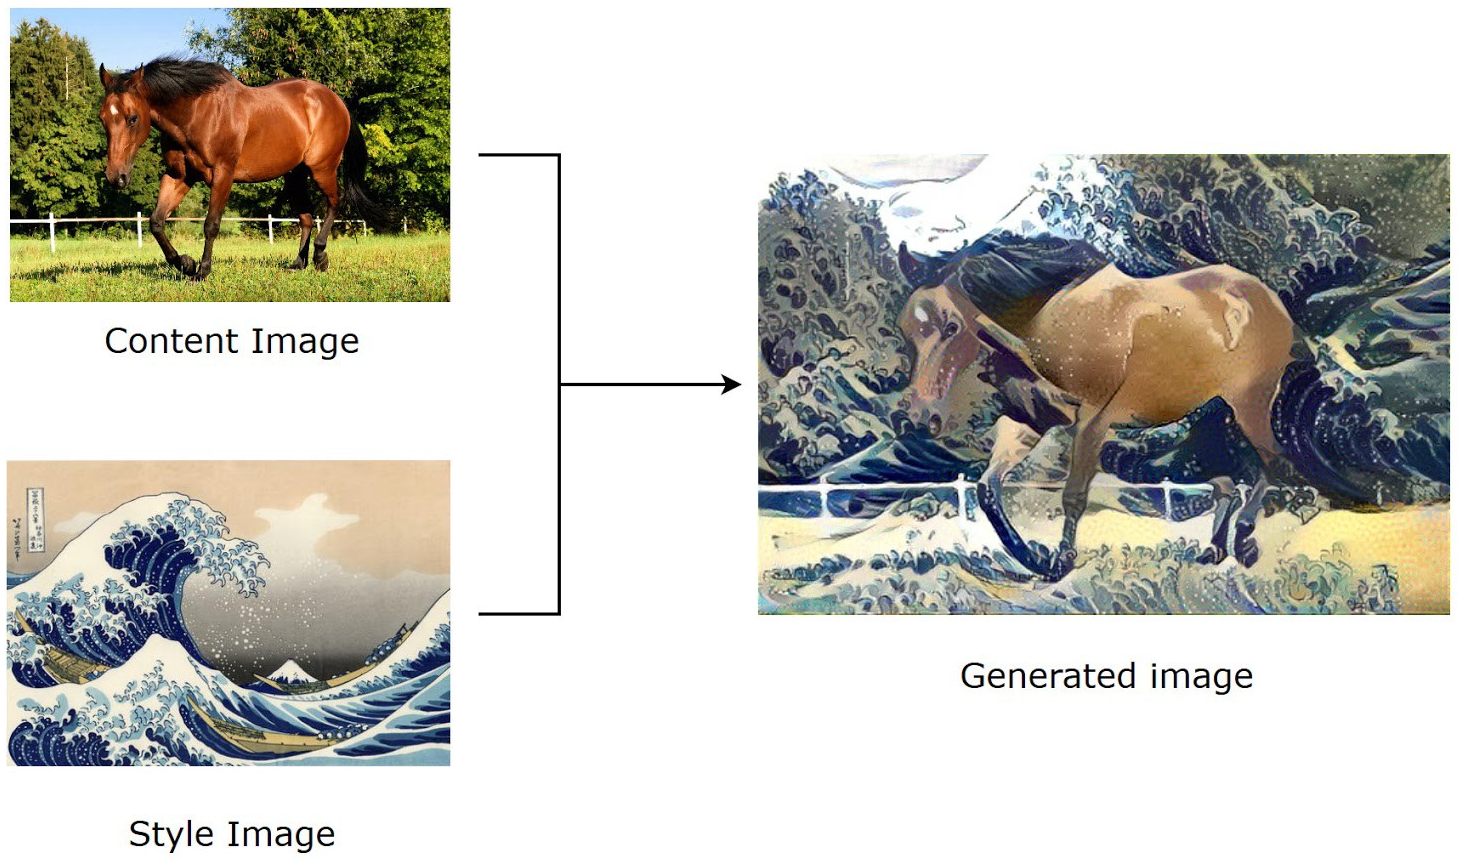
\includegraphics[width=0.45\textwidth]{resources/png/example.png}
        \caption{An example of neural style transfer product \cite{towardsdatascience.com}.}
        \label{fig:introduction.example}
    \end{figure}
    
    However, the rich domain of neural style transfer does not stop there, many other possible applications and extensions exist : modifying the style of a painting to make it look like a photo (and vice versa), modifying the style of certain elements of a photo (for example, transforming horses into zebras by applying a striped texture to them), transforming a summer landscape into a winter landscape, coloring an image, etc.\\
    
    The applications are many and varied. We have chosen to focus on the application of merging the style of an image and the content of another image.\\
    
    To do this, we first started by exploring the technique explained in the paper by Gatys et al. \cite{DBLP:journals/corr/GatysEB15a}. We tried to re-implement this technique ourselves, to improve it, and to vary the different parameters to understand how it works. This method is described in section \ref{methods.gatys} and its results are discussed in section \ref{results.gatys}.\\
    
    Secondly, we have looked at the CycleGAN (\emph{Cycle-Consistent Generative Adversarial Networks}) technique introduced in the paper by Zhu et al. \cite{DBLP:journals/corr/ZhuPIE17}. This technique, using generative adversarial networks, is very rich and allows many possible applications.\\
    
    An example of the application of this network of interest for this project is shown in Figure \ref{fig:introduction.example.cyclegan}.
    
    \begin{figure}[ht]
        \centering
        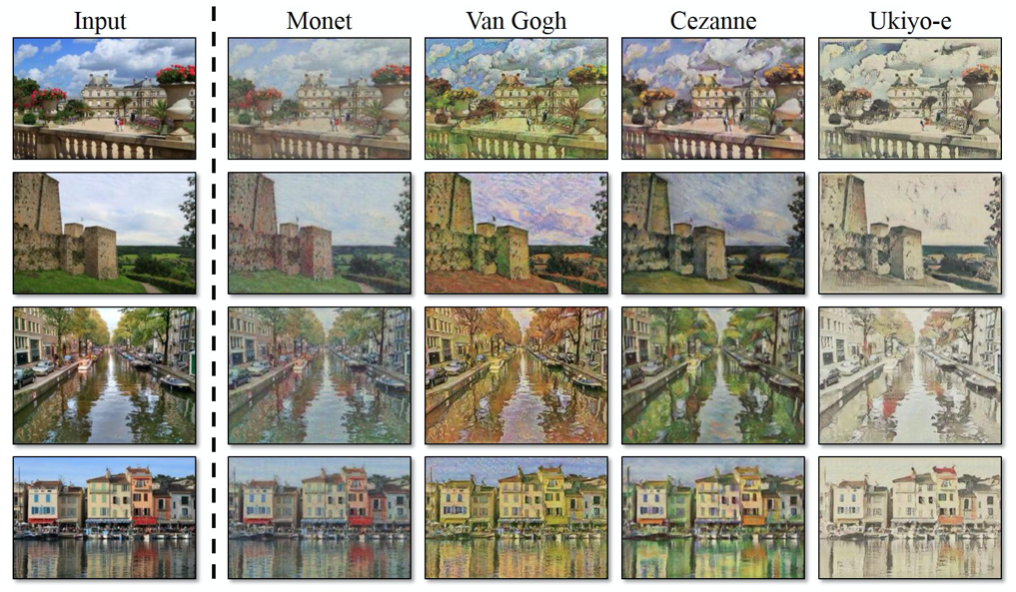
\includegraphics[width=0.45\textwidth]{resources/png/cyclegan-example.png}
        \caption{An example of neural style transfer produced by CycleGAN \cite{junyanz.github.io}.}
        \label{fig:introduction.example.cyclegan}
    \end{figure}
    
    We have also tried to re-implement it by ourselves and to vary its different elements. This method is described in section \ref{methods.zhu} and its results are discussed in section \ref{results.zhu}.\\
    
    Finally, we tried some extensions in order to dig deeper into the subject : use of different models, techniques to try to control colour, etc. These results are discussed in the corresponding sections of each method. The different difficulties encountered as well as our impressions of this work and our conclusion are explained in section \ref{discussion}.
    
    %%%%%%%%%%%%%%%%%%%%
    %%%%%%%%%%%%%%%%%%%%
    %%%%%%%%%%%%%%%%%%%%
    
    % ----- Related work ----- %
    
    % TO DO
    % -----
    % Research that is related to the considered problem
    
    \section{Related work}
    
    The field of neural style transfer and its applications are very rich. We have researched the literature to find out what the basic principles are, what the different techniques are and how they can be improved.\\
    
    We first based ourselves, as explained in the introduction, on the paper by Gatys et al. and on the paper by Zhu et al. :
    
    \begin{itemize}
        \item \cite{DBLP:journals/corr/GatysEB15a} - Paper by Gatys et al. : a paper that introduces a technique for neural style transfer using a network, such as VGG19, already trained.
        \item \cite{DBLP:journals/corr/ZhuPIE17} - Paper by Zhu et al. : a paper that introduces a technique, called CycleGAN, to perform unpaired image-to-image translation.
    \end{itemize}
    
    We then looked for some papers that could help us better understand the subject and improve our techniques. The field of \emph{style transfer} in deep learning is very rich and its literature very varied. We consulted a wide range of sources but we focused on papers that were most relevant to our implemented techniques.
    
    \begin{itemize}
        \item \cite{DBLP:journals/corr/JingYFYS17} - Paper by Jing et al. :  a paper that provides a comprehensive overview of the current progress towards neural style transfer.
        \item \cite{DBLP:journals/corr/GatysEBHS16} - Paper by Gatys et al. : a paper that follows their original one (\cite{DBLP:journals/corr/GatysEB15a}) and introduces several improvements concerning the results that can be obtained. Examples are the possibility to include bitmaps, to control the colour transfer and the scale.
        \item \cite{DBLP:journals/corr/JohnsonAL16} - Paper by Johnson et al. : a paper that takes advantage of \emph{perceptual loss functions} to design a style transfer algorithm. The latter is compared with the original technique of Gatys et al.
        \item \cite{DBLP:journals/corr/LedigTHCATTWS16} - Paper by Ledig et al. : a paper that presents SRGAN, a generative adversarial network (GAN) for image super-resolution (SR).
    \end{itemize}
    
    %%%%%%%%%%%%%%%%%%%%
    %%%%%%%%%%%%%%%%%%%%
    %%%%%%%%%%%%%%%%%%%%
    
    % ----- Methods ----- %
    
    % TO DO
    % -----
    % A clear and detailed description of the neural networks (architecture, training-parameters, loss function, data)
    
    \section{Methods}
    
    \subsection{Neural style transfer (Gatys et al.)}\label{methods.gatys}
    
    The method presented in this section is that of the original paper that introduced neural style transfer. Although style transfer previously existed in a field called \emph{non-photorealistic rendering} and were implemented through \emph{artistic rendering} algorithms \cite{DBLP:journals/corr/JingYFYS17}, they made no use of neural networks for the task and achieved limited performance and results.\\
    
    The paper \cite{DBLP:journals/corr/GatysEB15a} makes use of convolutional neural networks to tackle the task. Those networks are the most powerful when dealing with images since they are able to quickly and efficiently detect local and global correlations in an image. Thanks to filters implemented at each layer, features of the image can be gradually extracted in a feedforward manner. The outputs of each layer consist therefore in \emph{feature maps}, which are filtered versions of the input image.\\
    
    The authors decided to use networks that were pre-trained on object recognition tasks. Such a network creates a representation of the input image that makes the object information increasingly explicit during the treatment, and the content of the image is thus given more weight than the fine details. Higher-level layers contain high-level content while lower-level ones contain low-level details. High-level layers are thus used for content representation. On the other hand, the style is captured through correlations between the filter responses of different layers.\\
    
    The realization that made neural style transfer possible for the authors is that the style and content of an image are \emph{separable in a convolutional neural network}.\\
    
    As for the practical method proposed by the paper, they used the pretrained VGG19 network, consisting of 16 convolutional layers and 5 pooling ones. The responses in a layer $l$ being the features maps of that layer, they can be stored in a matrix $F^l \in \mathcal{R}^{N_l\times M_l}$, where $F_{ij}^l$ is the activation of the $i^{th}$ filter at position $j$ in layer $l$. $N_l$ is the number of distinct filters at layer $l$ and $M_l$ is the size of the feature map (height times width).\\ 
    
    The loss that the authors have used in their work is the following one :
    \begin{equation}\label{eq:gatys.loss}
        \mathcal{L}_{total}(\vec{p},\vec{a},\vec{x}) = \alpha \mathcal{L}_{content}(\vec{p},\vec{x}) + \beta \mathcal{L}_{style}(\vec{a},\vec{x})
    \end{equation}
    where
    \begin{equation}
        \mathcal{L}_{\text {content}}(\vec{p}, \vec{x}, l)=\frac{1}{2} \sum_{i, j}\left(F_{i j}^{l}-P_{i j}^{l}\right)^{2}
    \end{equation}
    and
    \begin{align}
        \mathcal{L}_{\text {style}}(\vec{a}, \vec{x}) &= \sum_{l=0}^{L} w_{l} E_{l}\nonumber\\
        &= \sum_{l=0}^{L} w_{l} \frac{1}{4 N_{l}^{2} M_{l}^{2}} \sum_{i, j}\left(G_{i j}^{l}-A_{i j}^{l}\right)^{2}
    \end{align}
    The parameter $p$ is the photograph (content image), $x$ is the constructed one and $a$ is the artwork (style image). Parameters $\alpha$ and $\beta$ are simply weighting factors controlling the tradeoff between style and content. The content loss is the mean square error between the response matrix of the content image and that of the constructed image, while the style loss is defined as the weighted sum of the mean square errors between the Gram matrices for the generated image and the style one, taken over all layers considered for the style. The \emph{Gram matrix} is a mathematical element that computes the correlation between the different filter responses for a given layer.
    
    \subsubsection{Network architecture}
    
    The authors used model VGG19 as a basis : VGG19 is a convolutional neural network which consists of 16 convolutional layers (to transform images to feature maps), 5 pooling layers (to reduce the dimensions of the data) and 3 fully connected ones (at the end where every neuron in one layer are connected to every neuron in another layer) where 19 layers are trainable (convolutional and fully connected layers). This model is used to classify images.\\
    
    The authors have modified this network by inserting layers to reconstruct the image. For the content, a layer was inserted after a convolutional layer. For the style, several layers have been added after convolutional layers (as explained previously, the style is rebuilt by calculating the correlation between the different features of different layers).\\
    
    The insertion of additional layers can be done in several different places. We have chosen this architecture as a starting point : \texttt{normalization}, \texttt{conv\_1}, \texttt{style\_loss\_1}, \texttt{relu\_1}, \texttt{conv\_2}, \texttt{style\_loss\_2}, \texttt{relu\_2}, \texttt{pool\_2}, \texttt{conv\_3}, \texttt{style\_loss\_3}, \texttt{relu\_3}, \texttt{conv\_4}, \texttt{content\_loss}, \texttt{style\_loss\_4}, \texttt{relu\_4}, \texttt{pool\_4}, \texttt{conv\_5}, \texttt{style\_loss\_5}. One can notice that the architecture is not complete. Indeed, all layers after the last style layer inserted have been put aside : they are no longer useful once the content and style have been reconstructed. This first \texttt{normalization} layer is used to normalize input images in order to fit VGG19.
    
    \subsubsection{Implementation}
    
    We tried to implement this technique by ourselves with PyTorch. In order to correct our errors and improve our implementation, we used the \cite{pytorch.org} and \cite{nextjournal.com} tutorials. Our basic implementation is as faithful as possible to the paper \cite{DBLP:journals/corr/GatysEB15a} : we have taken VGG19 and inserted the new layers at the same places, we have taken the same values of the $\alpha$ and $\beta$ parameters, etc. We varied all these parameters afterwards.\\
    
    We didn't need to build up a large dataset of images for this technique; we simply downloaded images of style and content from the Internet.\\
    
    Finally, we took advantage of the university's GPU cluster to get better results (larger images) faster.
    
    \subsection{CycleGAN (Zhu et al.)}\label{methods.zhu}
    
    CycleGAN is neural networks that allows to perform \emph{unpaired image-to-image translation}. As described on its official web page, "\emph{image-to-image translation is a class of vision and graphics problems where the goal is to learn the mapping between an input image and an output image using a training set of aligned image pairs.}" \cite{junyanz.github.io}. However, in many cases, paired images are not available. This technique has therefore been designed to support unpaired images.\\
    
    Paired images are images with a common context and common elements (for example, an image of horse in a field and an image of a zebra in the same position in more or less an identical field) while unpaired images are images that are not really the same (for example, an image of a horse in a field and an image of a zebra, not in the same position, not in the same size and not in a field).\\
    
    CycleGAN uses a \emph{generative adversarial network}.
    
    \subsubsection{Generative models}
    
    \emph{Generative models} are models capable of learning how to create data similar to the data they are provided with (training data). Intuitively, a model acting on data (e.g. writing good scientific articles) must have a good internal representation of this data. This internal representation could then be exploited to perform other tasks (e.g. classifying scientific articles).\\
    
    More practically, a generative model is a model that attempts to learn the joint probability distribution $P(x,y)$ between data $x$ and their label $y$ (where a non-generative model learns the conditional probability $P(y|x)$). Thus, the model would be able to generate a new sample $(x,y)$.
    
    \subsubsection{Generative adversarial networks}
    
    \emph{Generative adversarial networks} are models whose main idea is to put in competition two neural network models. One is called the \emph{generator} and is in charge of generating noisy data. The other is called the \emph{discriminator} and receives the training data and the noisy data from the generator and has to be able to distinguish between the two sources.\\
    
    An illustration of the structure of a generative adversarial networks is presented in Figure \ref{fig:methods.cyclegan.gan}.
    
    \begin{figure}[ht]
        \centering
        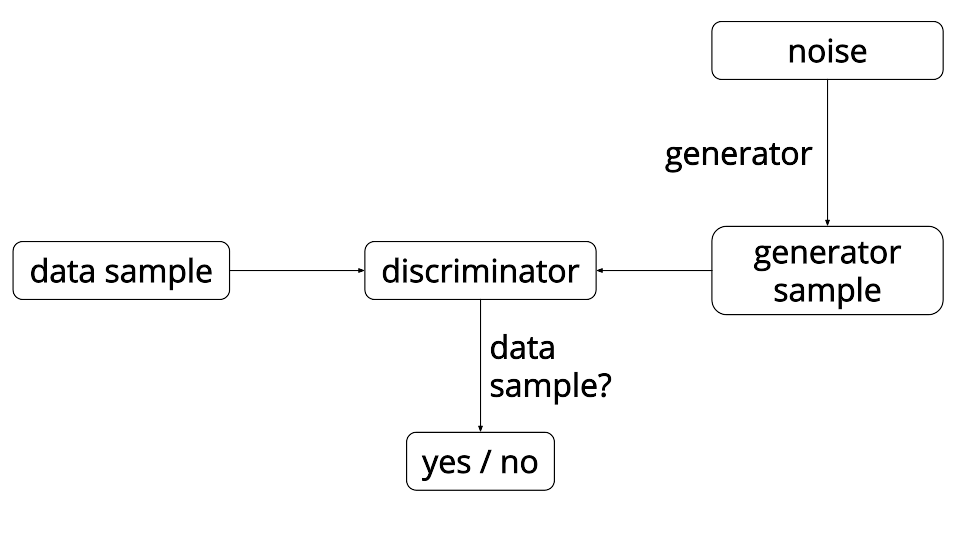
\includegraphics[width=0.45\textwidth]{resources/png/gan.png}
        \caption{Generative adversarial networks structure \cite{blog.aylien.com}.}
        \label{fig:methods.cyclegan.gan}
    \end{figure}
    
    As the training progresses, the generator produces less and less noisy data and the discriminator becomes better at distinguishing the source from the data it receives. The ultimate goal is to make the generator generate data that will be indistinguishable from the training data by the discriminator.\\
    
    In such a model, we can backpropagate gradient information from the discriminator back to the generator network, so the generator knows how to adapt its parameters in order to produce output data that can fool the discriminator.
    
    \subsubsection{CycleGAN}
    
    Coming back to the application of neural style transfer, the idea behind the use of a generative adversarial network is \emph{to learn a mapping between the input image and the output image}. However, this technique works for paired images. CycleGAN is a technique that works on unpaired images (or more generally, unpaired input data). For example, it will be able to transform a horse in a photo into a zebra (by applying a striped texture to it) without even needing a zebra image in the same position, with the same background, etc. (i.e. paired images of horse and zebra).\\
    
    The operating principle of CycleGAN is as follows : let one set of images (for example, images of horses) in an $X$ domain and another different set of images (for example, images of zebras) in a $Y$ domain. The goal is to obtain, via training, a mapping $G : X \rightarrow Y$ and a mapping $F : Y \rightarrow X$. Mathematically, $G$ and $F$ should be inverse to each other and both mapping should be bijections. This hypothesis being made, $G$ and $F$ are trained simultaneously via a \emph{cycle consistency loss} that encourages $F(G(x)) = x$ and $G(F(y)) = y$.\\
    
    The creators of CycleGAN have in fact exploited the fact that a translation must be "\emph{cycle consistent}" using this technique. Concretely, this means, for example, that if a sentence is translated from English into French, the re-translation of the freshly obtained French sentence into English should give the original sentence.\\
    
    Exploiting this property avoids problems such as \emph{mode collapse} : the model could generate an image which is in the domain of $Y$, and which would therefore be validated by the discriminator, without having any link with the domain $X$ (for example, generating an image of a zebra that is always abd always the same and does not look anything like the image of the original horse).\\
    
    In total, the model contains two loss functions : an \emph{adversarial loss function} (since it is a generative adversarial model) and a \emph{cycle consistent loss function} (to take into account the cycle consistent property).\\
    
    The adversarial loss function is defined as
    \begin{align}
        \mathcal{L}_{\mathrm{GAN}}\left(G, D_{Y}, X, Y\right)&=\mathbb{E}_{y \sim p_{\text {data }}(y)}\left[\log D_{Y}(y)\right]\nonumber\\
        &+\mathbb{E}_{x \sim p_{\text {data }}(x)}\left[\log \left(1-D_{Y}(G(x))\right]\right.
    \end{align}
    where $D_Y$ is a discriminant which aims to distinguish the images ${y}$ from the translated images ${G(x)}$. They also consider the same loss for $D_X$.\\
    
    The cycle consistent loss function is defined as
    \begin{align}
        \mathcal{L}_{\text {cyc }}(G, F) &=\mathbb{E}_{x \sim p_{\text {data }}(x)}\left[\|F(G(x))-x\|_{1}\right]\nonumber\\
        &+\mathbb{E}_{y \sim p_{\text {data }}(y)}\left[\|G(F(y))-y\|_{1}\right]
    \end{align}
    taking into account that the result must satisfy the \emph{forward cycle consistency} ($x\rightarrow G(x)\rightarrow F(G(x))\approx x$) and the \emph{backward cycle consistency} ($y\rightarrow F(y)\rightarrow G(F(y))\approx y$).\\
    
    An illustration of the cycle consistent loss is shown in Figure \ref{fig:methods.cyclegan.cycleconsistentloss}.\\
    
    \begin{figure}[ht]
        \centering
        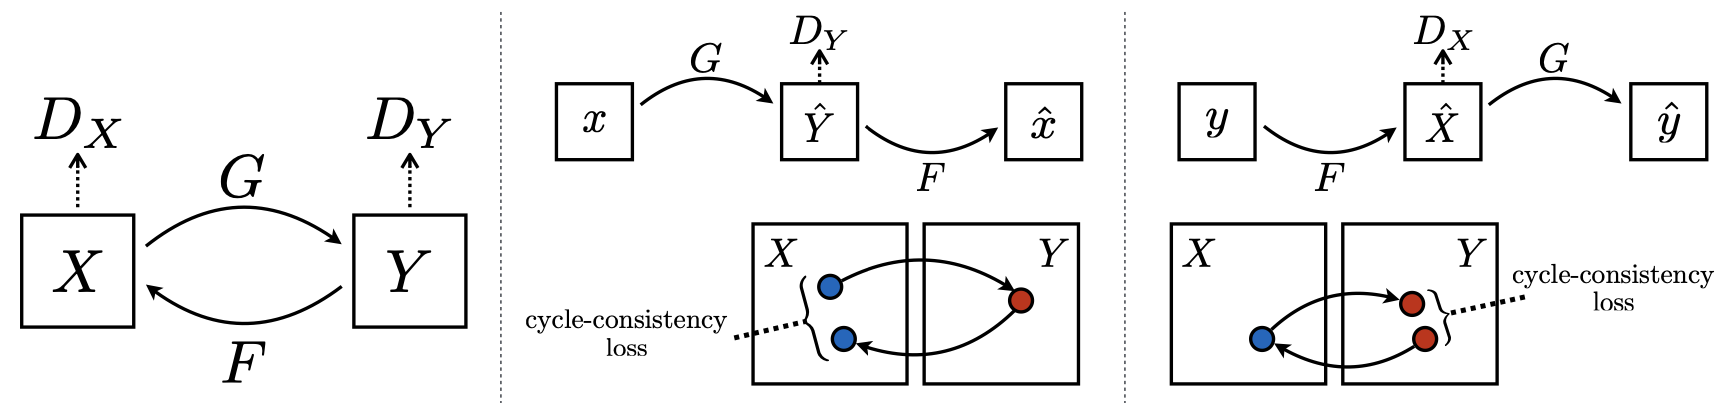
\includegraphics[width=0.45\textwidth]{resources/png/cycle-consistent-loss.png}
        \caption{Cycle consistent loss \cite{DBLP:journals/corr/ZhuPIE17}}
        \label{fig:methods.cyclegan.cycleconsistentloss}
    \end{figure}
    
    Finally, the total loss function that the model tries to minimize is defined as
    \begin{align}
        \mathcal{L}\left(G, F, D_{X}, D_{Y}\right) &= \mathcal{L}_{\mathrm{GAN}}\left(G, D_{Y}, X, Y\right)\nonumber\\
        &+ \mathcal{L}_{\mathrm{GAN}}\left(F, D_{X}, Y, X\right)\nonumber\\
        &+ \lambda \mathcal{L}_{\mathrm{cyc}}(G, F)
    \end{align}
    where $\lambda$ controls the relative importance of the two objectives.
    
    \subsubsection{Network architectures}
    
    Concerning generator architectures, authors of CycleGAN use architecture from Johnson et al. \cite{DBLP:journals/corr/JohnsonAL16} : 6 residual blocks for $128 \times 128$ training images and 9 residual blocks for $256 \times 256$ or higher-resolution training images.\\
    
    Concerning the discriminator architectures, they use a $70 \times 70$ PatchGAN.
    
    \subsubsection{Implementation}
    
    In order to implement the CycleGAN, we decided to not base ourselves upon a tutorial but instead to try to recreate the models and its training from the paper \cite{DBLP:journals/corr/ZhuPIE17} itself. The network architecture is referenced in the fourth section of this paper and makes reference to the network used in another paper \cite{DBLP:journals/corr/JohnsonAL16}. The exact architecture of the networks of this paper being given in the supplementary and using the discriminator architecture of \cite{DBLP:journals/corr/LedigTHCATTWS16}. We therefore tried to implement our network based on these sources and finished doing so before realizing that the exact architectures of CycleGan were given in the appendix of their paper, located after the sources. We thus used that source to modify the networks created to have the same basis as them. For the generator, we did not modify anything since the architecture we used and modified based on their comment in their own implementation was the same as the one provided in their appendix. For the discriminators, however, we had to modify our architecture since they did not mention that the kernel sizes were of 4, and so we went with the kernel size of 3 referenced by the original paper they based upon, and they used a stride of 2 for all layers, which was not the case in \cite{DBLP:journals/corr/LedigTHCATTWS16}. The number of blocks they used also differed.\\
    
    Finally, after having implemented the network, we went to their GitHub repository for the paper and compared our architecture and theirs, to make sure everything was correct. The only modification we had to make was change some reflection padding to simple padding with 0. They mentioned in their paper they used reflection padding to reduce artifacts but it was not done for all convolutional layers, so we modified that.\\
    
    After the network architectures, we had to acquire a dataset of images and paintings. To do so, we used a bash script found on their GitHub repository that downloads the same datasets as they used in their research. We decided to use landscapes and Monet paintings for the two domains of interest. We also had to create a custom data loader that would return an image of both domain when called, and to do so we looked into PyTorch documentation and StackOverflow questions.\\
    
    For the optimizer, we reused the same as the authors, and created a learning rate scheduler based on what they wrote in their paper.
    
    %%%%%%%%%%%%%%%%%%%%
    %%%%%%%%%%%%%%%%%%%%
    %%%%%%%%%%%%%%%%%%%%
    
    % ----- Results ----- %
    
    % TO DO
    % -----
    % Qualitative analysis : could include examples of generated images, correct vs wrong predictions, ...
    % Quantitative analysis : general overview of final performance, loss curves, comparison table with error-bars, ...
    
    \section{Results}
    
    \subsection{Neural style transfer (Gatys et al.)}\label{results.gatys}
    
    In order to better understand this technique to obtain the best possible results, we tried to vary the different parameters (and hyperparameters) controlling the model. These are listed below :
    
    \begin{itemize}
        \item input image;
        \item model used;
        \item architecture of the model used;
        \item number of steps (epochs);
        \item weights;
        \item added layers.
    \end{itemize}
    
    We discuss each result obtained in a qualitative way by comparing the image obtained with the initial images and in a quantitative way by discussing the loss functions. Since this is a very visual, and therefore very subjective, application, there are few quantitative criteria to discuss. The quality of the result obtained depends very much on the user and his visual feeling.
    
    \subsubsection{Input image}
    
    The input image is the image that will be generated by the model. It can be initialized in two different ways : either by taking a copy of the content image, or by taking a white noise version of the content image. According to the literature, these two possibilities are equivalent. We have therefore tried both versions.\\
    
    We chose the \emph{Arc de Triomphe} (Paris) as the reference content image (\ref{fig:input.image.ref.content}) and a painting as the reference style image (\ref{input.image.ref.style}). These two images will be used in further discussions. Obviously, the parameters that give good results for these images will not necessarily give good results for all images. We will discuss this point later.
    
    \begin{figure}[ht]
        \centering
        \begin{subfigure}[b]{0.22\textwidth}
            \centering
            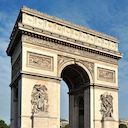
\includegraphics[width=\textwidth]{resources/png/inputs/paris.png}
            \caption{Content image}
            \label{fig:input.image.ref.content}
        \end{subfigure}
        \hfill
        \begin{subfigure}[b]{0.22\textwidth}
            \centering
            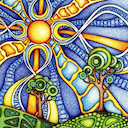
\includegraphics[width=\textwidth]{resources/png/inputs/sun-trees.png}
            \caption{Style image}
            \label{input.image.ref.style}
        \end{subfigure}
        \caption{Reference images}
    \end{figure}
    
    For this first test, we kept the original implementation, faithful to paper \cite{DBLP:journals/corr/GatysEB15a}, with 300 epochs. The results obtained are presented in Figure \ref{fig:input.image.variations}.
    
    \begin{figure}[ht]
        \centering
        \begin{subfigure}[b]{0.22\textwidth}
            \centering
            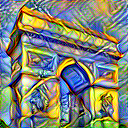
\includegraphics[width=\textwidth]{resources/png/inputs/sun-trees-paris-copy.png}
            \caption{Start with copy of content image}
        \end{subfigure}
        \hfill
        \begin{subfigure}[b]{0.22\textwidth}
            \centering
            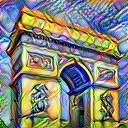
\includegraphics[width=\textwidth]{resources/png/inputs/sun-trees-paris-noisy.png}
            \caption{Start with noisy content image}
        \end{subfigure}
        \caption{Input image variations}
        \label{fig:input.image.variations}
    \end{figure}
    
    As can be seen, the results obtained are very similar. However, starting with a copy of the content image seems to give smoother results for the majority of cases. For this reason, we will choose to start with a copy of the content image afterwards.
    
    \subsubsection{Model used}
    
    The authors used a pre-trained version of the VGG19 model. This version already has a set of defined weights for a better classification and therefore better results for style transfer. We tried to run the algorithm with the non pre-trained VGG19 model to compare the two versions. The results obtained are shown in Figure \ref{fig:model.pretrained.variations}.
    
    \begin{figure}[ht]
        \centering
        \begin{subfigure}[b]{0.22\textwidth}
            \centering
            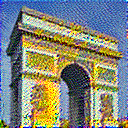
\includegraphics[width=\textwidth]{resources/png/model/sun-trees-paris-notpretrained.png}
            \caption{Not pre-trained model}
        \end{subfigure}
        \hfill
        \begin{subfigure}[b]{0.22\textwidth}
            \centering
            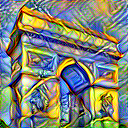
\includegraphics[width=\textwidth]{resources/png/model/sun-trees-paris-pretrained.png}
            \caption{Pre-trained model}
        \end{subfigure}
        \caption{VGG19 model variations}
        \label{fig:model.pretrained.variations}
    \end{figure}
    
    We can easily observe that the pre-trained model gives much better results than the non pre-trained model. This result seems logical since the pre-trained model allows a less good extraction of the features of each image and therefore a much worse reconstruction and mix of content and style of each image.\\
    
    We tried to increase the number of epochs of the algorithm with the non pre-trained model, but the results obtained are systematically much lower than the results with the pre-trained model. To obtain better results, we should have trained the VGG19 model beforehand. Since image classification was not the main subject of our project, we worked directly with the pre-trained model afterwards.
    
    \subsubsection{Architecture of the model used}
    
    The original architecture of VGG19 has max pooling layers. The authors suggest in their paper to replace these max pooling layers by average pooling layers in order to obtain more appealing results. We have therefore compared the results with these two types of layers (Figure \ref{fig:model.architecture.variations}).
    
    \begin{figure}[ht]
        \centering
        \begin{subfigure}[b]{0.22\textwidth}
            \centering
            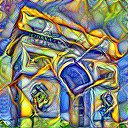
\includegraphics[width=\textwidth]{resources/png/architecture/sun-trees-paris-maxpool.png}
            \caption{Max pooling layers}
        \end{subfigure}
        \hfill
        \begin{subfigure}[b]{0.22\textwidth}
            \centering
            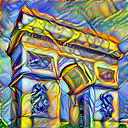
\includegraphics[width=\textwidth]{resources/png/architecture/sun-trees-paris-avgpool.png}
            \caption{Average pooling layers}
        \end{subfigure}
        \caption{VGG19 model architecture variations}
        \label{fig:model.architecture.variations}
    \end{figure}
    
    At first glance, both results seem to be very good. However, in general, some images give very bad results with average pooling layers (while results with max pooling layers are always very good). We have therefore observed the evolution of the loss functions (Figure \ref{fig:model.architecture.loss}).
    
    \begin{figure}[ht]
        \centering
        \begin{subfigure}[b]{0.22\textwidth}
            \centering
            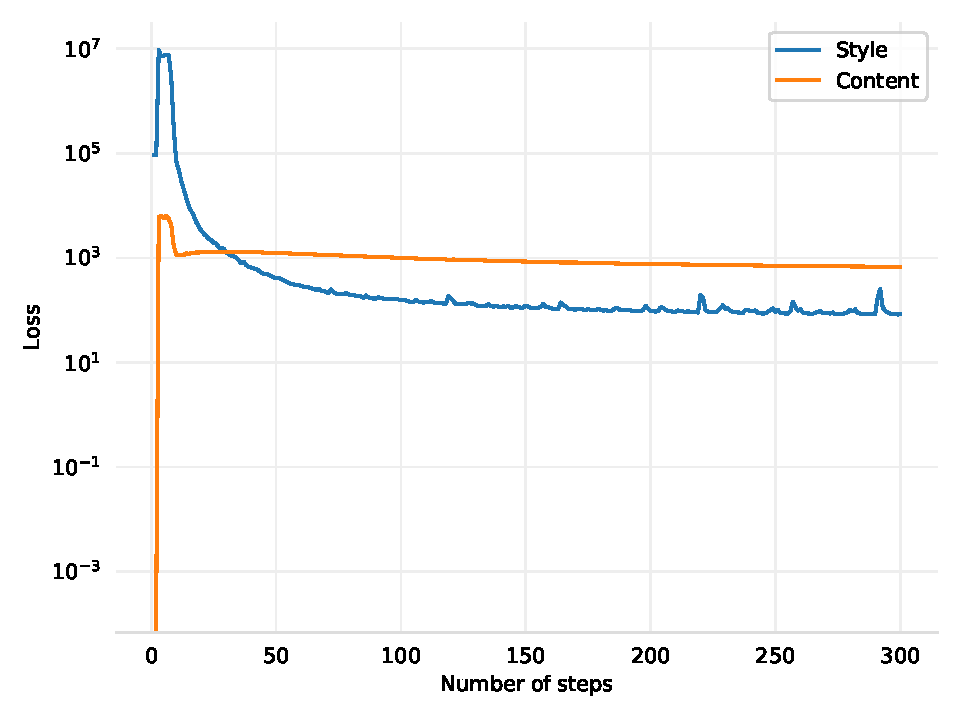
\includegraphics[width=\textwidth]{resources/pdf/architecture/sun-trees-paris-maxpool.pdf}
            \caption{Max pooling layers}
        \end{subfigure}
        \hfill
        \begin{subfigure}[b]{0.22\textwidth}
            \centering
            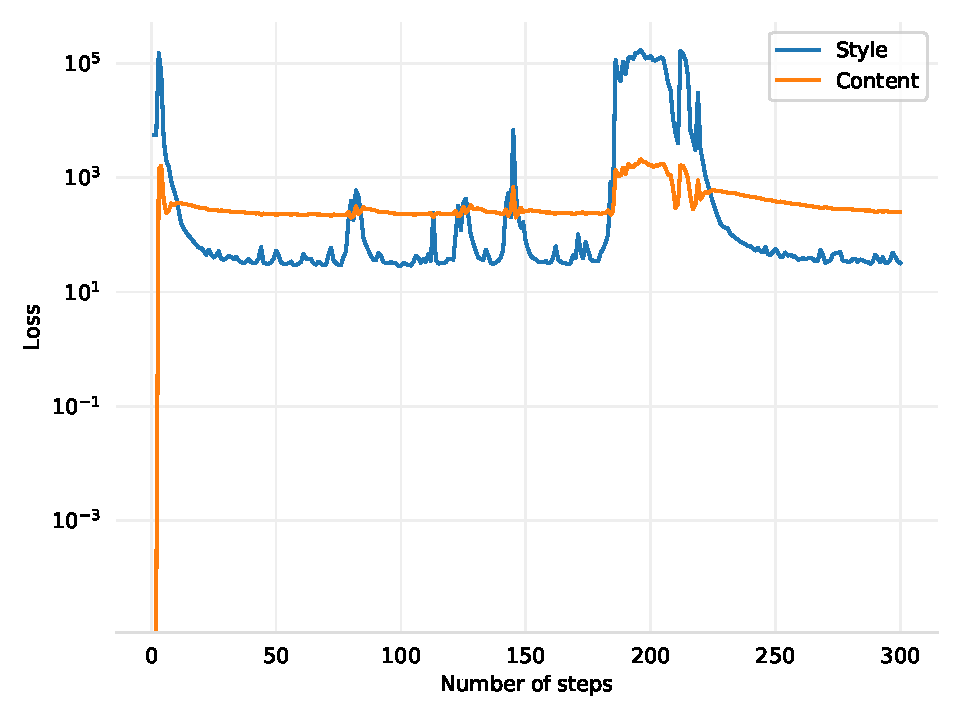
\includegraphics[width=\textwidth]{resources/pdf/architecture/sun-trees-paris-avgpool.pdf}
            \caption{Average pooling layers}
        \end{subfigure}
        \caption{VGG19 model architecture loss functions}
        \label{fig:model.architecture.loss}
    \end{figure}
    
    We observe that in the case of an architecture with average pooling layers, the loss functions (and especially the one concerning the content) vary strongly during the epochs while in the case of max pooling layers, the loss functions remain stable. This could explain the very bad results obtained on some images with average pooling layers.\\
    
    To overcome this, we have added a \emph{scheduler} (with a step size of 50 and a gamma parameter of 0.3) when working with average pooling layers. This scheduler allows to reduce the learning rate during epochs, and thus to reduce the variations of the loss functions. We then restarted the algorithm with this scheduler (Figure \ref{fig:model.architecture.loss.scheduler}).
    
    \begin{figure}[ht]
        \centering
        \begin{subfigure}[b]{0.22\textwidth}
            \centering
            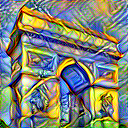
\includegraphics[width=\textwidth]{resources/png/architecture/sun-trees-paris-avgpool-scheduler.png}
            \caption{Transformed input image}
        \end{subfigure}
        \hfill
        \begin{subfigure}[b]{0.22\textwidth}
            \centering
            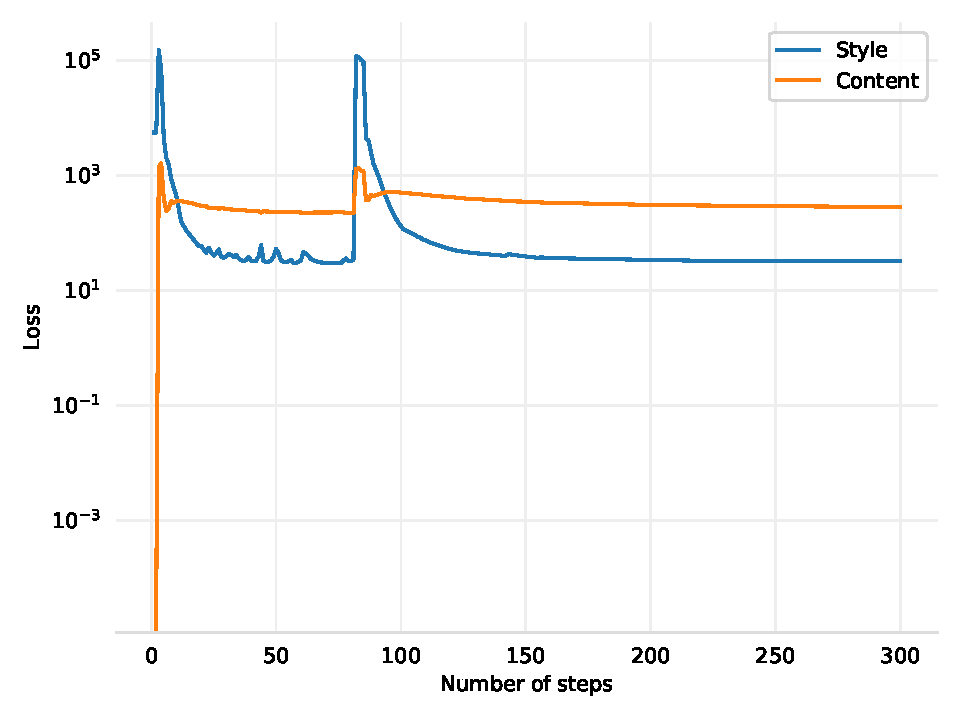
\includegraphics[width=\textwidth]{resources/pdf/architecture/sun-trees-paris-avgpool-scheduler.pdf}
            \caption{Loss functions}
        \end{subfigure}
        \caption{Average pooling layers with scheduler (VGG19)}
        \label{fig:model.architecture.loss.scheduler}
    \end{figure}
    
    We observe that the scheduler seems to be efficient since the variations of the loss functions have almost completely disappeared. In general, the results that were previously bad have turned out to be very good with the scheduler. The images obtained with average pooling layer seem to be smoother. So we kept this type of layer (with a scheduler).
    
    \subsubsection{Number of steps (epochs)}
    
    By default, we have set the number of steps (epochs) to 300. The results are obtained quickly and seem to be good. When we observe the loss functions (Figure \ref{fig:model.architecture.loss.scheduler} for example), we realize that they stabilize quite quickly (after about 300 epochs).
    
    In order to confirm this result, we run the algorithm by increasing the number of epochs to 1000. The result obtained is shown in Figure \ref{fig:number.steps.variations}.
    
    \begin{figure}[ht]
        \centering
        \begin{subfigure}[b]{0.22\textwidth}
            \centering
            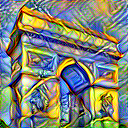
\includegraphics[width=\textwidth]{resources/png/steps/sun-trees-paris-300.png}
            \caption{300 epochs}
        \end{subfigure}
        \hfill
        \begin{subfigure}[b]{0.22\textwidth}
            \centering
            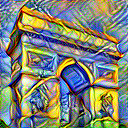
\includegraphics[width=\textwidth]{resources/png/steps/sun-trees-paris-1000.png}
            \caption{1000 epochs}
        \end{subfigure}
        \caption{Number of steps variations}
        \label{fig:number.steps.variations}
    \end{figure}
    
    As expected, the two results are exactly the same. Indeed, considering the evolution of the loss functions (Figure \ref{fig:number.steps.loss.functions}) per 1000 epochs, we can confirm that they stabilize quite quickly. We have therefore set the number of epochs to 300 by default.
    
    \begin{figure}[ht]
        \centering
        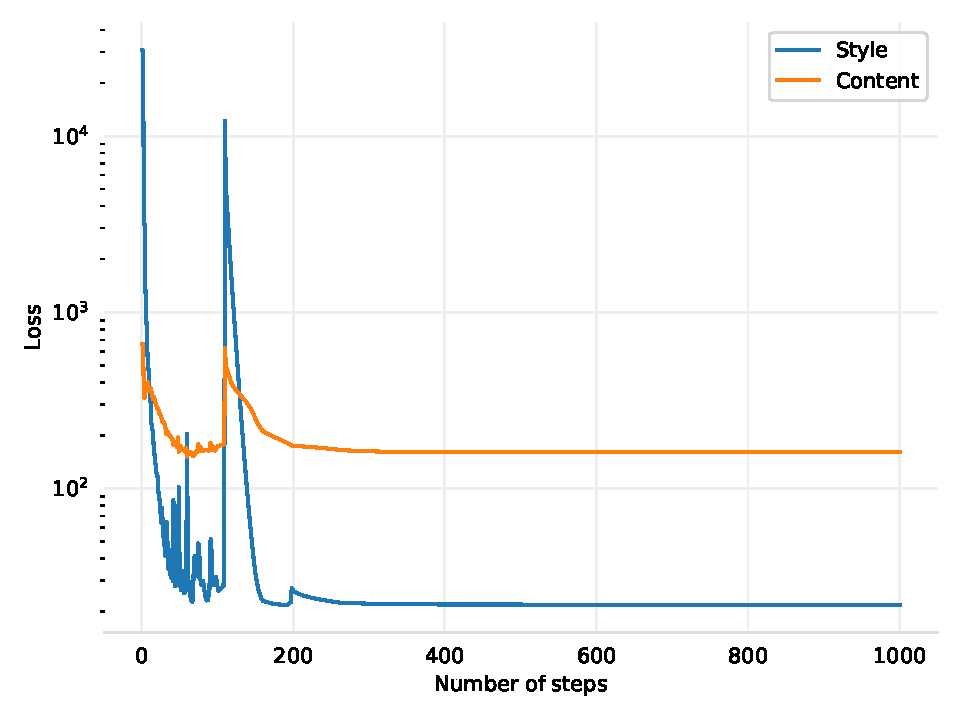
\includegraphics[width=0.45\textwidth]{resources/pdf/steps/sun-trees-paris-1000.pdf}
        \caption{Loss functions for 1000 epochs}
        \label{fig:number.steps.loss.functions}
    \end{figure}
    
    \subsubsection{Weights}
    
    It is possible to vary the $\alpha$ and $\beta$ weights in the loss function \eqref{eq:gatys.loss}. These weights are used to distribute the style and content of the resulting image. In their paper, the authors use an $\alpha/\beta$ ratio equals to $10^{-4}$. We have tried several ratios to observe the variations of the results obtained (Figure \ref{fig:weights.ratio}).
    
    \begin{figure}[ht]
        \centering
        \begin{subfigure}[b]{0.13\textwidth}
            \centering
            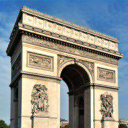
\includegraphics[width=\textwidth]{resources/png/weights/sun-trees-paris-10-2.png}
            \caption{$10^{-2}$}
        \end{subfigure}
        \hfill
        \begin{subfigure}[b]{0.13\textwidth}
            \centering
            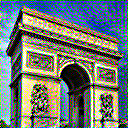
\includegraphics[width=\textwidth]{resources/png/weights/sun-trees-paris-10-3.png}
            \caption{$10^{-3}$}
        \end{subfigure}
        \hfill
        \begin{subfigure}[b]{0.13\textwidth}
            \centering
            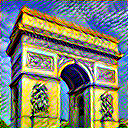
\includegraphics[width=\textwidth]{resources/png/weights/sun-trees-paris-10-4.png}
            \caption{$10^{-4}$}
        \end{subfigure}
        \begin{subfigure}[b]{0.13\textwidth}
            \centering
            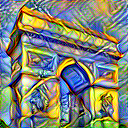
\includegraphics[width=\textwidth]{resources/png/weights/sun-trees-paris-10-5.png}
            \caption{$10^{-5}$}
        \end{subfigure}
        \hfill
        \begin{subfigure}[b]{0.13\textwidth}
            \centering
            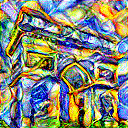
\includegraphics[width=\textwidth]{resources/png/weights/sun-trees-paris-10-6.png}
            \caption{$10^{-6}$}
        \end{subfigure}
        \hfill
        \begin{subfigure}[b]{0.13\textwidth}
            \centering
            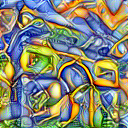
\includegraphics[width=\textwidth]{resources/png/weights/sun-trees-paris-10-7.png}
            \caption{$10^{-7}$}
        \end{subfigure}
        \caption{Results for different values of ratio $\alpha/\beta$}
        \label{fig:weights.ratio}
    \end{figure}
    
    We observe that if the ratio is too high ($10^{-2}$), the result is not influenced at all by the style image and, on the contrary, if the ratio is too low ($10^{-7}$), the style totally takes over the result. A suitable ratio seems to be around $10^{-5}$. This result is of course highly dependent on the images and the expected result : a low contrast style image with dull colors will require a very low ratio to appear while a very bright and colorful style image will appear with a higher ratio. In general, the $10^{-5}$ ratio seems to give good results for all image combinations. We have therefore kept this value.\\
    
    We note that the $\alpha$ value is much smaller than the $\beta$ value. Indeed, the base image being a copy of the content image, it is not necessary to greatly modify it from a content point of view.\\
    
    We also tried to assign a weight to each layer added to rebuild the style image. Indeed, the authors mention in their paper that "\emph{[...] when matching the style representations up to higher layers in the network, local images structures are matched on an increasingly large scale, leading to a smoother and more continuous visual experience. Thus, the visually most appealing images are usually created by matching the style representation up to the highest layers in the network. [...]}" \cite{DBLP:journals/corr/GatysEB15a}. We therefore varied the influence of the different layers used to rebuild the style image by assigning them different weights (Figure \ref{fig:weights.style.layers}).

    \begin{figure}[ht]
        \centering
        \begin{subfigure}[b]{0.13\textwidth}
            \centering
            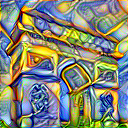
\includegraphics[width=\textwidth]{resources/png/weights/sun-trees-paris-equals-weights.png}
            \caption{$w = [1, 1, 1, 1, 1]$}
        \end{subfigure}
        \hfill
        \begin{subfigure}[b]{0.13\textwidth}
            \centering
            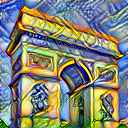
\includegraphics[width=\textwidth]{resources/png/weights/sun-trees-paris-linear-decreasing-weights.png}
            \caption{$w = [1, .8, .6, .4, .2]$}
        \end{subfigure}
        \hfill
        \begin{subfigure}[b]{0.13\textwidth}
            \centering
            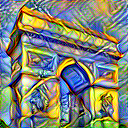
\includegraphics[width=\textwidth]{resources/png/weights/sun-trees-paris-high-decreasing-weights.png}
            \caption{$w = [.75, .5, .2, .2, .2]$}
        \end{subfigure}
        \caption{Style layers' weights variations}
        \label{fig:weights.style.layers}
    \end{figure}
    
    We get different results, but each one is very good. We find that, logically, by assigning less weight to the different style layers (especially the last ones), we obtain results where the style is less marked. Again, the ratings are very subjective and depend on the user's desired results.
    
    \subsubsection{Added layers}
    
    For this section, we have obtained more meaningful results by using another style image. We have therefore replaced our reference style image with the painting shown in Figure \ref{added.layers.ref.style}.
    
    \begin{figure}[ht]
        \centering
        \begin{subfigure}[b]{0.22\textwidth}
            \centering
            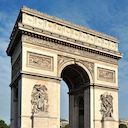
\includegraphics[width=\textwidth]{resources/png/inputs/paris.png}
            \caption{Content image}
        \end{subfigure}
        \hfill
        \begin{subfigure}[b]{0.22\textwidth}
            \centering
            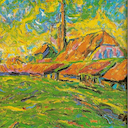
\includegraphics[width=\textwidth]{resources/png/inputs/church.png}
            \caption{Style image}
            \label{added.layers.ref.style}
        \end{subfigure}
        \caption{New reference images}
    \end{figure}
    
    The authors mention in their paper that the layers considered to reconstruct the image of content and the image of style have a significant influence on the result. The content image is rebuilt after a convolutional layer and the style image is rebuilt based on a correlation of several layers. We tried to put them at different places inside the VGG19 model in order to observe the influence on the result obtained abd try to find the best configuration.\\
    
    Visiblement j'ai pas pris le bon style je vais les refaire et adapter la discussion que j'avais préparée (pas grave, suffisait de préciser que tu changeais d'image de style, mais comme tu veux)
    
    \begin{figure}[ht]
        \centering
        \begin{subfigure}[b]{0.1\textwidth}
            \centering
            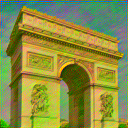
\includegraphics[width=\textwidth]{resources/png/layers/conv1_conv1.png}
            \caption{conv1 conv1}
        \end{subfigure}
        \hfill
        \begin{subfigure}[b]{0.1\textwidth}
            \centering
            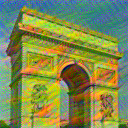
\includegraphics[width=\textwidth]{resources/png/layers/conv3_conv1.png}
            \caption{conv3 conv1}
        \end{subfigure}
        \hfill
        \begin{subfigure}[b]{0.1\textwidth}
            \centering
            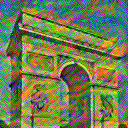
\includegraphics[width=\textwidth]{resources/png/layers/conv5_conv1.png}
            \caption{conv5 conv1}
        \end{subfigure}
        \hfill
        \begin{subfigure}[b]{0.1\textwidth}
            \centering
            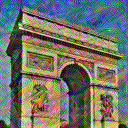
\includegraphics[width=\textwidth]{resources/png/layers/conv9_conv1.png}
            \caption{conv9 conv1}
        \end{subfigure}
        \begin{subfigure}[b]{0.1\textwidth}
            \centering
            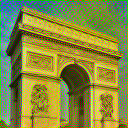
\includegraphics[width=\textwidth]{resources/png/layers/conv1_conv3.png}
            \caption{conv1 conv3}
        \end{subfigure}
        \hfill
        \begin{subfigure}[b]{0.1\textwidth}
            \centering
            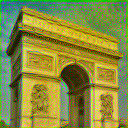
\includegraphics[width=\textwidth]{resources/png/layers/conv1_conv5.png}
            \caption{conv1 conv5}
        \end{subfigure}
        \hfill
        \begin{subfigure}[b]{0.1\textwidth}
            \centering
            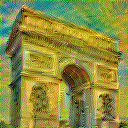
\includegraphics[width=\textwidth]{resources/png/layers/conv1_conv9.png}
            \caption{conv1 conv9}
        \end{subfigure}
        \hfill
        \begin{subfigure}[b]{0.1\textwidth}
            \centering
            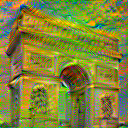
\includegraphics[width=\textwidth]{resources/png/layers/conv3_conv9.png}
            \caption{conv3 conv9}
        \end{subfigure}
        \caption{Influence of the position of the construction layers}
        \label{fig:added.layers}
    \end{figure}
    
    \subsubsection{Final results}
    
    We have tried to explore the technique of Gatys et al. and to vary its different parameters in order to better understand it. In summary, we observed that taking as input image a copy of the content image gives smoother results; a pre-trained model logically gives better results; average pooling layers (with a scheduler) give, on average, better results; 300 epochs seem to be sufficient and that, finally, a ratio of $10^{-5}$ between the weight of the content and the weight of the style seems to be good on average. Other parameters such as where new layers are added and the weights assigned to these layers depend very strongly on the input images.\\
    
    We applied the algorithm to a whole series of images, adjusting the parameters as best we could according to the different discussions made previously. Our results are presented in Figure \ref{fig:final.results.gatys}.
    
    \begin{figure*}[ht]
        \centering
        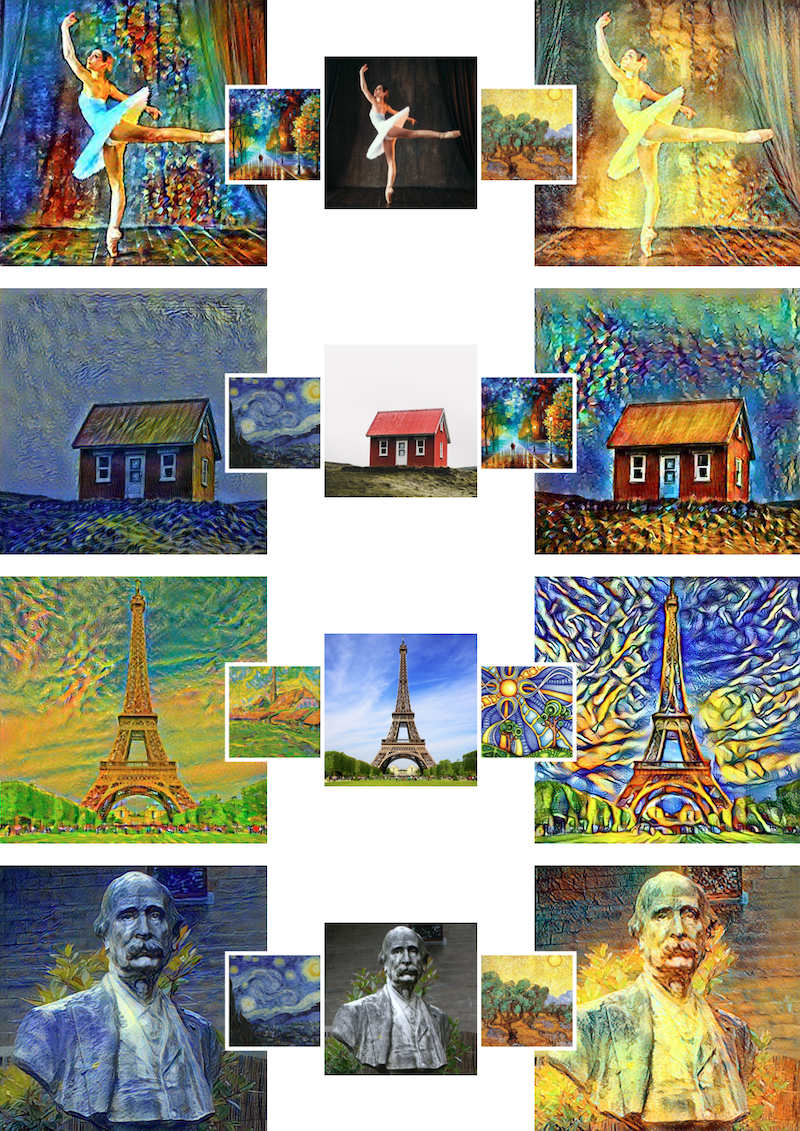
\includegraphics[width=0.85\textwidth]{resources/png/gatys-final.png}
        \caption{Some results obtained with Gatys et al. technique}
        \label{fig:final.results.gatys}
    \end{figure*}
    
    \subsection{CycleGAN (Zhu et al.)}\label{results.zhu}
    
    to do
    
    %%%%%%%%%%%%%%%%%%%%
    %%%%%%%%%%%%%%%%%%%%
    %%%%%%%%%%%%%%%%%%%%
    
    % ----- Discussion ----- %
    
    % TO DO
    % -----
    % A critical discussion of the performance of the neural network, analysis of the potential limitations, tips for future work
    
    \section{Discussion}\label{discussion}
    
    \subsection{Neural style transfer (Gatys et al.)}
    
    Our implementation of the technique of Gatys et al. is quite faithful to the original paper. Although inspired by tutorials, we have added our own personal touch in order to re-implement certain aspects and to better understand it.\\
    
    The results we get seem good at first glance. However, the field of style transfer is very rich and has evolved a lot since the publication of the paper by Gatys et al. \cite{DBLP:journals/corr/GatysEB15a} and many methods that drastically improve the results have emerged. We have focused here on the basic principles but a whole range of improvements could have been possible. Our model has its limitations in that, given the rapidly stabilizing loss functions, we cannot get much better results just by playing with the basic parameters.\\
    
    We used a pre-trained model for this project. We didn't bother trying to train the model by ourselves as it would have been very time consuming and not really related to our topic. However, training a model (e.g. VGG19) with a wide range of artistic images (paintings, etc.) might have led, maybe, to better results.\\
    
    Finally, we realized how much deep learning techniques, even modern ones, require a lot of work on parameters and training in order to obtain suitable results. Moreover, a series of parameters that give suitable results for one image will not give suitable results for another; it is difficult to generalize the model.\\
    
    We are satisfied with the results we are achieving. It is difficult to judge their quality from a quantitative point of view in view of this very subjective application, but nevertheless, from a qualitative point of view, the results are very correct.
    
    %%%%%%%%%%%%%%%%%%%%
    %%%%%%%%%%%%%%%%%%%%
    %%%%%%%%%%%%%%%%%%%%
    
    % ----- References ----- %
    
    \newpage
    
    \bibliographystyle{unsrt}
    \bibliography{references.bib}
    \nocite{*}
\end{document}
